\documentclass[11pt]{amsart}
\usepackage{amsmath, amssymb, amsthm, amsfonts,enumitem,fontawesome,mathtools,framed,caption}
\usepackage[T1]{fontenc}
\usepackage{newpxtext,newpxmath,tabu}

\usepackage[colorlinks = true, allcolors = blue!60!black]{hyperref}
\usepackage[margin = 1.25in]{geometry}
\usepackage{tikz,tikz-3dplot}
\usetikzlibrary{math}

\pgfdeclarelayer{background}
\pgfdeclarelayer{foreground}
\pgfsetlayers{background,main,foreground} 

\theoremstyle{plain}
\newtheorem{theorem}{Theorem}[section]
\newtheorem*{theorem*}{Theorem}
\newtheorem{corollary}[theorem]{Corollary}
\newtheorem{lemma}[theorem]{Lemma}
\newtheorem*{lemma*}{Lemma}
\newtheorem{proposition}[theorem]{Proposition}
\newtheorem{problem}{Problem}
\newtheorem{fact}[theorem]{Fact}


\theoremstyle{definition}
\newtheorem{definition}[theorem]{Definition}
\newtheorem*{definition*}{Definition}
\newtheorem{example}{Example}
\newtheorem*{exercise*}{Exercise}

\newtheorem{remark}[theorem]{Remark}
\newtheorem*{remark*}{Remark}
\newtheorem{conjecture}[theorem]{Conjecture}
\newtheorem*{conjecture*}{Conjecture}
\newtheorem*{setup}{Setup}
\newtheorem*{notation}{Notation}
\theoremstyle{remark}
\newtheorem{claim}{Claim}
\renewcommand{\theclaim}{\arabic{claim}}
\newenvironment{proofclaim}{\begin{proof}[Proof of Claim]\renewcommand{\qedsymbol}{$\lozenge$}}{\end{proof}}


\newcommand{\complex}{\mathbb{C}}
\newcommand{\naturals}{\mathbb{N}}
\newcommand{\integers}{\mathbb{Z}}
\newcommand{\rationals}{\mathbb{Q}}
\newcommand{\reals}{\mathbb{R}}



\DeclareMathOperator{\Sym}{Sym} 
\DeclareMathOperator{\Alt}{Alt} 
\DeclareMathOperator{\GL}{GL} 
\DeclareMathOperator{\SL}{SL}
\DeclareMathOperator{\AGL}{AGL} 
\DeclareMathOperator{\PGL}{PGL} 
\DeclareMathOperator{\PSL}{PSL} 
\DeclareMathOperator{\Proj}{P} 

\newcommand{\symtetra}{\textsc{Tetra}}
\newcommand{\rsymtetra}{\textsc{Tetra}^+}
\newcommand{\symcube}{\textsc{Cube}}
\newcommand{\rsymcube}{\textsc{Cube}^+}
\newcommand{\symicosa}{\textsc{Icosa}}
\newcommand{\rsymicosa}{\textsc{Icosa}^+}

\DeclareMathOperator{\Aut}{Aut}
\DeclareMathOperator{\End}{End} 
\DeclareMathOperator{\charac}{char}  
\DeclareMathOperator{\Fix}{Fix} 
\DeclareMathOperator{\id}{id} 
\DeclareMathOperator{\Stab}{Stab} 
\DeclareMathOperator{\Orb}{Orb} 



\begin{document}
\title[Permutation Groups]{Topics in Permutation Groups\\[7pt] {\footnotesize A short seminar series}}
\author{Joshua Wiscons}
\address{Department of Mathematics and Statistics\\
California State University, Sacramento\\
Sacramento, CA 95819, USA}
\email{joshua.wiscons@csus.edu}
\date{\today}

\maketitle

\tableofcontents

% % % % % % % % % % % % % % % % % % % % % % % % % % % % % % % % % % % % % % % % % % % % % % % % % 
% % % % % % % % % % % % % % % % % % % % % % % % % % % % % % % % % % % % % % % % % % % % % % % % % 
% Section
% % % % % % % % % % % % % % % % % % % % % % % % % % % % % % % % % % % % % % % % % % % % % % % % % 
% % % % % % % % % % % % % % % % % % % % % % % % % % % % % % % % % % % % % % % % % % % % % % % % % 
%\section{Introduction}\label{S:introduction}
These (in progress!) notes are being prepared for a six-part seminar series on permutation groups in Spring 2022 at California State University, Sacramento. The seminar is meant to be casual, example driven, hopefully fun, and accessible to anyone having completed a first course in linear algebra, though exposure to groups will help. 

\newpage
% % % % % % % % % % % % % % % % % % % % % % % % % % % % % % % % % % % % % % % % % % % % % % % % % 
% % % % % % % % % % % % % % % % % % % % % % % % % % % % % % % % % % % % % % % % % % % % % % % % % 
% Section
% % % % % % % % % % % % % % % % % % % % % % % % % % % % % % % % % % % % % % % % % % % % % % % % % 
% % % % % % % % % % % % % % % % % % % % % % % % % % % % % % % % % % % % % % % % % % % % % % % % % 
\section{A First Example}\label{S:first.example}
Let's start by exploring symmetries of a familiar object. We'll also introduce notation as we go.

\begin{example}\label{exam:Tetra}
Consider a regular tetrahedron, like the \href{https://en.wikipedia.org/wiki/Pyraminx}{Pyraminx} (pictured below). One way to represent the various symmetries is to consider how each symmetry permutes the vertices, so let's label them as follows

\begin{center}
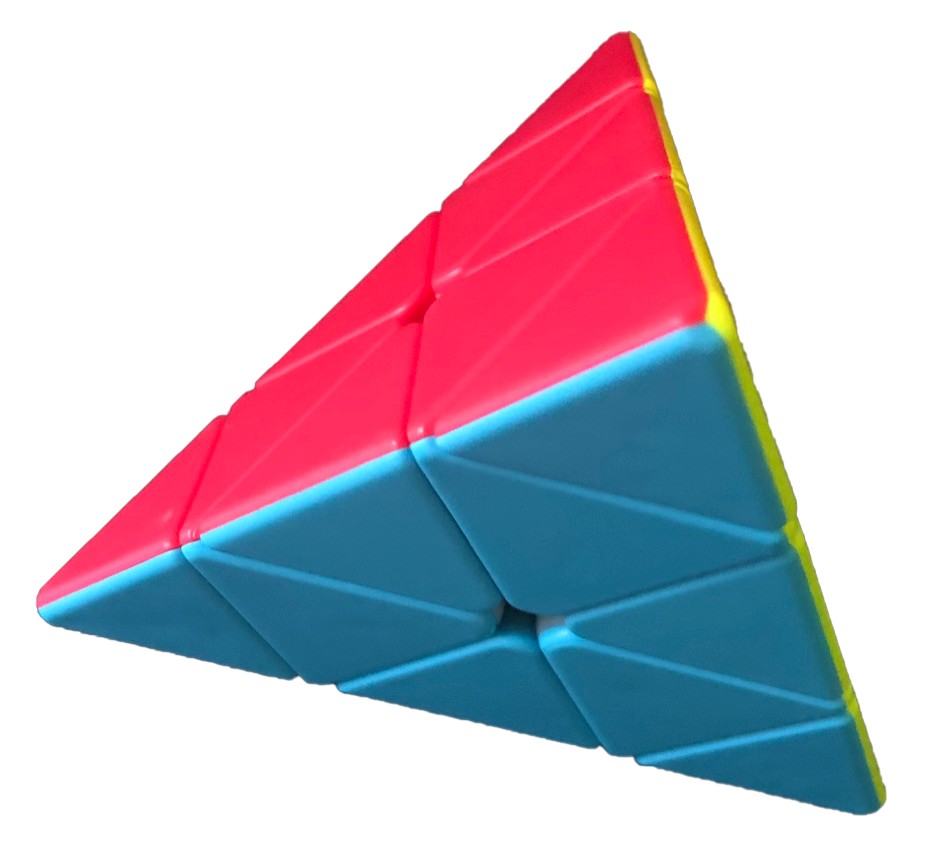
\includegraphics[height=1.3in,angle =20,origin=c]{tetra.png}\hspace{0.75in}
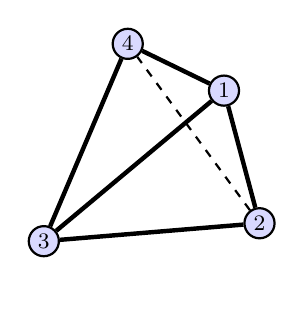
\begin{tikzpicture}[vertex/.style={circle,draw=black,fill=blue!15,thick,inner sep=1.5pt},ultra thick,rotate around x=-10,rotate around z=-5,scale = 1,baseline=-50pt]
\footnotesize
\node[vertex,anchor = 0] (v1) at (1,1,1) {$1$};
\node[vertex,anchor = 0] (v2) at (1,-1,-1) {$2$};
\node[vertex,anchor = 0] (v4) at (-1,1,-1) {$4$};
\node[vertex,anchor = 0] (v3) at (-1,-1,1) {$3$};

\draw (v1) -- (v2);\draw (v1) -- (v3);\draw (v1) -- (v4);
\draw (v2) -- (v3);\draw[dashed,thick] (v2) -- (v4);
\draw (v3) -- (v4);
\end{tikzpicture}
\end{center}


Let $\symtetra$ denote the collection of \emph{all} symmetries of this object and $\rsymtetra$ denote just the \emph{rotational} symmetries. We will view each element of $\symtetra$ (and $\rsymtetra$) as a permutation of the set $\{1,2,3,4\}$. The collection of \emph{all} permutations of $\{1,2,3,4\}$ will be denoted $\Sym(4)$, so with this notation we have $\rsymtetra\subseteq \symtetra\subseteq \Sym(4)$. Let's pause to define and introduce notation for $\Sym(X)$ generally.

\begin{definition*}
Let $X$ be a set. The \textbf{symmetric group} on $X$, denoted $\Sym(X)$, is the set of all permutations of $X$. When $X = \{1,2,\ldots, n\}$, we  write $\Sym(n)$ in place of $\Sym(X)$. We also adopt the following notation.
\begin{itemize}
\item The identity permutation will be denoted $\id_X$ (or just $\id$), so $\id_X(x)=x$ for all $x\in X$.
\item For $\sigma,\tau\in \Sym(X)$,  $\sigma\tau$ denotes composition of $\sigma$ and $\tau$, so $\sigma\tau(x) = \sigma(\tau(x))$ for all $x\in X$. 
\item For $\sigma\in \Sym(X)$ and $n\in \naturals$, $\sigma^n$ denotes the composition of $\sigma$ with itself $n$-times, and $\sigma^{-n}$ denotes the composition of $\sigma^{-1}$ with itself $n$-times.
\end{itemize}
We may refer to $\sigma\tau$ as the \emph{product} of $\sigma$ and $\tau$, but in $\Sym(X)$ this means composition.
\end{definition*}

Let's resume our investigation of the tetrahedron, and list some  elements of $\rsymtetra$. As we do, we'll introduce additional notation for writing permutations. 

If we hold the top vertex $1$, we can rotate the remaining ones by $120^\circ$ to obtain the permutation $\gamma$ defined via $\gamma(1) = 1$, $\gamma(2) = 3$, $\gamma(3) = 4$, and $\gamma(4) = 2$. We  occasionally write permutations in \href{https://en.wikipedia.org/wiki/Permutation#Two-line_notation}{two-line notation} as below; the top row lists the inputs while the bottom lists the corresponding outputs.
\[\gamma = \begin{pmatrix}
1 & 2 & 3 & 4\\
1 & 3 & 4 & 2\\
\end{pmatrix}\]

More often, we will write permutations in so-called (disjoint) \href{https://en.wikipedia.org/wiki/Permutation#Cycle_notation}{cycle notation}, which  will be ``defined'' via various examples. Writing $\gamma$ using cycle notation yields $\gamma = (234)$. This is read left to right and indicates that a given number is mapped by $\gamma$ to the number immediately to the right, cycling back to the beginning when the rightmost parenthesis is encountered. We can picture this as $2\rightarrow 3\rightarrow 4\rightarrow 2$. Any number not appearing (like $1$ in this case) is left fixed by the permutation. Because of the cyclical nature of this notation, there are various ways to write $\gamma$ in this notation: $\gamma = (234) = (342) = (423)$.

Let's look for more symmetries. If we continue to hold the top vertex and rotate $120^\circ$ again (for a total of $240^\circ$), we have the permutation $\gamma^2 = \gamma\gamma$. In two line notation, 
\[\gamma^2 = \begin{pmatrix}
1 & 2 & 3 & 4\\
1 & 4 & 2 & 3\\
\end{pmatrix},\]
and in cycle notation, $\gamma^2 = (243)$. Yet another rotation by $120^\circ$, returns the shape to the starting configuration, so $\gamma^3 = \id$. Also note, that we could have initially rotated by $-120^\circ$, which is the inverse of $\gamma$ (i.e. $\gamma^{-1}$), but this does not yield a new permutation since $\gamma^{-1} = (432) = (243) = \gamma^2$.

Now, this time, let's hold vertex $2$, and rotate by $120^\circ$. Depending on your point of view, there are two options, but one of them is $\delta = (134)$. And rotating in the same direction by another $120^\circ$, yields $\delta^2 = (143)$. We can further consider holding the vertex $3$ or $4$ while rotating. So far, we've found the following rotational symmetries of the tetrahedron:
\[\{\id, (234), (243), (134), (143), (124), (142), (123), (132)\} \subseteq \rsymtetra.\]
There are more. Imagine the line $\ell$ connecting the midpoint of the edge $\{1,4\}$ (from vertex $1$ to $4$) with the midpoint of the edge $\{2,3\}$ (from vertex $2$ to $3$); then let $\alpha$ be the rotation of the tetrahedron by $180^\circ$ about the line $\ell$.  In two-line notation, we find that 
\[\alpha = \begin{pmatrix}
1 & 2 & 3 & 4\\
4 & 3 & 2 & 1\\
\end{pmatrix},\]
and in cycle notation, we have $\alpha = (14)(23)$. Performing $180^\circ$ rotations about the other two lines that connect pairs of ``opposite edges'', we find that $\rsymtetra$ also contains $(12)(34)$ and $(13)(24)$. So now we have that 
\[
\begin{Bmatrix}
\id,(12)(34), (13)(24), (14)(23),  \\
(234), (243), (134), (143), (124), (142), (123), (132)
\end{Bmatrix}
\subseteq \rsymtetra.\]

What else could be in $\rsymtetra$? Well, $\Sym(4)$ contains 12 more permutations that we have not encountered yet. Six of the remaining permutations move only two vertices while fixing the others, e.g. $\tau = (12)$; these permutations are called \textbf{transpositions} (since they transpose two numbers and leave the remaining unaltered). Now, $\tau$ does  represent a symmetry of the tetrahedron, namely \emph{reflection} through the plane that contains the edge $\{3,4\}$ and is orthogonal to the edge $\{1,2\}$. However, $\tau$  is not a \emph{rotational} symmetry because a nontrivial rotational symmetry can only fix a vertex that is on the axis of rotation, and due to the structure of the tetrahedron, at most one vertex can lie on an axis of rotation that produces a symmetry. Similarly, we find that the other transpositions are in $\symtetra$ but \emph{not} $\rsymtetra$, so 
\[\{(12), (13), (14), (23), (24), (34)\} \subseteq \symtetra - \rsymtetra.\]
The only permutations in $\Sym(4)$ we have not yet considered are the so-called $4$-cycles, such as $\sigma = (1234)$. Notice that $\sigma\in \symtetra$ since $\sigma = (12)(23)(34)$, so it can be realized by performing three reflections in a row. However, $\sigma$ is not a rotational symmetry. To see this, note that any rotation that moves vertex $2$ to $3$ and vertex $3$ to $4$ must have an axis of rotation orthogonal to \emph{both} of the edges $\{2,3\}$ and $\{3,4\}$, implying that the axis of rotation runs through vertex $1$, so $1$ would have to remain fixed. Thus, $\sigma$ is not a rotational symmetry. Similarly, we see that each $4$-cycle is in $\symtetra$ but \emph{not}  $\rsymtetra$. In conclusion, we've found  
\begin{align*}
\symtetra &= \Sym(4)\\
\rsymtetra &= \begin{Bmatrix}
\id,(12)(34), (13)(24), (14)(23),  \\
(234), (243), (134), (143), (124), (142), (123), (132)
\end{Bmatrix}
\end{align*}

Incidentally, although we already knew that the composition of any two symmetries of the tetrahedron was another symmetry, we can now directly verify that the composition of any two \emph{rotational} symmetries is another \emph{rotational} symmetry (e.g. $\gamma\delta = (234)(134) = (14)(23) = \alpha$).
\end{example}

% % % % % % % % % % % % % % % % % % % % % % % % % % % % % % % % % % % % % % % % % % % % % % % % % 
% % % % % % % % % % % % % % % % % % % % % % % % % % % % % % % % % % % % % % % % % % % % % % % % % 
% Section
% % % % % % % % % % % % % % % % % % % % % % % % % % % % % % % % % % % % % % % % % % % % % % % % % 
% % % % % % % % % % % % % % % % % % % % % % % % % % % % % % % % % % % % % % % % % % % % % % % % % 
\section{Permutation groups}\label{S:permgroups}

In this section, we'll formally introduce permutation groups and the related notion of group actions. We'll also see more examples (in addition to $\symtetra$ and $\rsymtetra$); this includes the important family of alternating groups as well as the symmetry group of a cube. The section concludes with a couple of fundamental concepts in the study of permutation groups: orbits and stabilizers.

\begin{definition*}
Let $X$ be a set. A subset $G \subseteq \Sym(X)$ is called a \textbf{subgroup} of $\Sym(X)$ if all of the following hold:
\begin{itemize}
\item{} [\textsc{closure under the identity}] $\id \in G$;
\item{} [\textsc{closure under composition}] if $\alpha,\beta \in G$, then $\alpha\beta \in G$;
\item{} [\textsc{closure under inverses}] if $\alpha \in G$, then $\alpha^{-1} \in G$.
\end{itemize}
In this case, we say $G$ is a \textbf{permutation group} on $X$.
\end{definition*}

\begin{example}
As can be seen from Example~\ref{exam:Tetra}, $\symtetra$ and $\rsymtetra$ can both be viewed as permutation groups on $\{1,2,3,4\}$.
\end{example}


% % % % % % % % % % % % % % % % % % % % % % % % % % % % % % % % % % % % % % % % % % % % % % % % % 
% Subsection
% % % % % % % % % % % % % % % % % % % % % % % % % % % % % % % % % % % % % % % % % % % % % % % % % 
\subsection{The alternating group}

Recall that an element $\tau \in \Sym(X)$ of the form $\tau = (ij)$  is called a transposition (for any $i\neq j \in X$). Let's explore how to decompose a given permutation into a product (i.e.~composition) of transpositions.

\begin{example}\label{exam.DecomposeTranspositions}
Consider the permutation $\alpha = (12345)$. After computing various products of transpositions, one might notice that  $\alpha$ can be written as  $\alpha = (12)(23)(34)(45)$ or $\alpha = (15)(14)(13)(12)$ or something else. Since $(ij)(ij) = \id$ for each transposition $(ij)$, one sees that there are a lot of ways to write $\alpha$ as a product of transpositions; for example, $\alpha = (12)(23)(34)(45)(12)(12)$ or $\alpha = (67)(12)(23)(34)(45)(67)$ (assuming in the latter case that we are working in $\Sym(n)$ for $n\ge 7$). 

What about the permutation $\beta = (12345)(6789)$? We can decompose $\beta$ similar to before by treating each of the cycles $(12345)$ and $(6789)$ separately: $\beta = (12)(23)(34)(45)(67)(78)(89)$. And again, there are many ways to decompose $\beta$ into a product of transpositions. 
\end{example}

Abstracting our technique in the previous example, we get the following result; the proof is left as an exercise. In group-theoretic parlance, it says that each finite symmetric group is \emph{generated} by its transpositions. 

\begin{lemma*}
Every permutation in $\Sym(n)$ can be written as a product of transpositions.
\end{lemma*}

\begin{definition*}
Let $\sigma \in \Sym(n)$. We call $\sigma$ an \textbf{odd} permutation if it can be written as a product of an odd number of transpositions. Similarly, we call $\sigma$  an \textbf{even} permutation if it can be written as a product of an even number of transpositions.
\end{definition*}

Looking back to Example~\ref{exam.DecomposeTranspositions}, the permutation $\alpha$ was even; while $\beta$ was odd. Notice that although there were several ways to write $\alpha$ as a product of transpositions, \emph{every} way we came up with used an even number. It turns our that this was no coincidence.

\begin{lemma*}
Every permutation in $\Sym(n)$ is either even or odd, but not both.
\end{lemma*}
\begin{proof}[Proof idea.]
One first observation to make is that it suffices to prove $\id$ is (even but) not odd. Indeed, suppose we know that $\id$ is not odd. Towards a contradiction, assume an arbitrary $\sigma$ is both even and odd. Then we can write $\sigma = \tau_1\cdots\tau_{k} = \rho_1\cdots\rho_{\ell}$ where $k$ is even, $\ell$ is odd, and each $\tau_i$ and each $\rho_j$ is a transposition. This implies  $\id = \sigma\sigma^{-1} = \tau_1\cdots\tau_{k}\rho_{\ell}^{-1}\cdots\rho_1^{-1}$. As the inverse of a transposition is itself, $\id  = \tau_1\cdots\tau_{k}\rho_{\ell}\cdots\rho_1$, implying that $\id$ is odd (since  $k$ is even and $\ell$ is odd), a contradiction.

So, it remains to show $\id$ is not odd. This is where most of the effort is, and we will simply refer out---sorry! A quick search of the internet will turn up various proofs of this lemma, but one nice (and  detailed) outline of the proof can be found in Dana Ernst's abstract algebra book, see \cite[Theorem 4.103]{ErD-Algebra}.
\end{proof}

Notice that composing two even permutations results in another even permutation. Moreover, the previous ``proof'' discussed that $\id$ is even, and it also indicated that a permutation has the same parity as its inverse. Combining this, we arrive at the following fundamental theorem-definition.

\begin{theorem*}
Let $\Alt(n)$ denote the collection of all even permutations in $\Sym(n)$. Then $\Alt(n)$ is a subgroup of $\Sym(n)$; it is called the \textbf{alternating group}.
\end{theorem*}

\begin{example}
A concise summary of Example~\ref{exam:Tetra} is that if we view the elements of $\symtetra$ as permutations of $\{1,2,3,4\}$, then $\symtetra = \Sym(4)$ and $\rsymtetra = \Alt(4)$. 

Note that, technically, the elements of $\symtetra$ operate on the entire tetrahedron, not just the vertices. Thus $\symtetra$ is not literally equal to $\Sym(4)$, so it is  more precise to use the language of \href{https://en.wikipedia.org/wiki/Isomorphism}{isomorphisms} and write $\symtetra \cong \Sym(4)$ and $\rsymtetra \cong \Alt(4)$. But in general, we won't much worry about this.
\end{example}

% % % % % % % % % % % % % % % % % % % % % % % % % % % % % % % % % % % % % % % % % % % % % % % % % 
% Subsection
% % % % % % % % % % % % % % % % % % % % % % % % % % % % % % % % % % % % % % % % % % % % % % % % % 
\subsection{One group, many actions}

When analyzing a permutation group $G$ on some set $X$, it is  important to keep in mind that $G$ may very well also permute other sets, and simultaneously studying the various ``actions'' of $G$ can be quite advantageous. For example, $\symtetra$ is first and foremost acting on the points of $\mathbb{R}^3$ (in a way that preserves the tetrahedron); however, the way we studied $\symtetra$ was via its action on the \emph{vertices} of the tetrahedron. However, $\symtetra$ also permutes the \emph{edges} of the tetrahedron as well as the \emph{faces} and various other related sets of objects. 

Let's formalize the notion of an ``action'', and then see how to leverage this idea with an example.

\begin{remark*}
In what follows, we will occasionally use a phrase like ``let $G$ be a group.'' This can be taken to mean that $G$ is a permutation group on some set $X$, but we don't care what $X$ is. The point is that sometimes we only want to focus on how the elements of the group $G$ interact with each other as opposed to how they permute the elements of $X$. If you've encountered the definition of an abstract group, then you could alternatively interpret ``let $G$ be a group'' as ``let $G$ be an abstract group.''
\end{remark*}

\begin{definition*}
Let $G$ be a group. We say $G$ \textbf{acts} on a set $Y$ if each $g\in G$ defines a function $Y \rightarrow Y : y \mapsto g\cdot y$ in such a way that 
\begin{enumerate}
\item for all $g,h\in G$ and all $y\in Y$, $g\cdot (h\cdot y) = (gh)\cdot y$, and
\item for all $y\in Y$, $\id\cdot y = y$.
\end{enumerate}
We say the action is \textbf{faithful} if the only element of $G$ satisfying $g\cdot y = y$ for all $y\in Y$ is $\id$.
\end{definition*}

In reading the definition, one should think of the notation $g\cdot y$ as $g(y)$. In what follows, we will often use the notation $g\cdot y$ in place of $g(y)$ for permutation groups too.

\begin{remark*}
If $G$ acts on a set $Y$, then the definition  implies that each element of $G$ can be viewed as a \emph{permutation} of $Y$. However, it is possible for different elements of $G$ to represent the same permutation of $Y$. (We'll see this in a later example.) 

Now, if the action is faithful, then it can be shown that different elements of $G$ always act as different permutations of $Y$, so in this case, we can view $G$ as a permutation group on $Y$ (even though $G$ may also be a permutation group on some other set $X$). Technical note: the sentence ``we can view $G$ as a permutation group on $Y$'' really means that ``$G$ is isomorphic to a permutation group on $Y$''.
\end{remark*}

\begin{example}\label{exam:Cube}
Let's work out the symmetries of a cube like \href{https://en.wikipedia.org/wiki/Rubik\%27s_Revenge}{Rubik's Revenge} (pictured below). Let $\symcube$ denote the collection of all symmetries of the cube, and let $\rsymcube$ denote the rotational symmetries. As in Example~\ref{exam:Tetra}, $\symcube$ as acts \emph{faithfully} on the $8$ vertices of the cube, so after labeling the vertices (as below), we may view $\symcube$ as a subgroup of $\Sym(8)$. 

\begin{center}
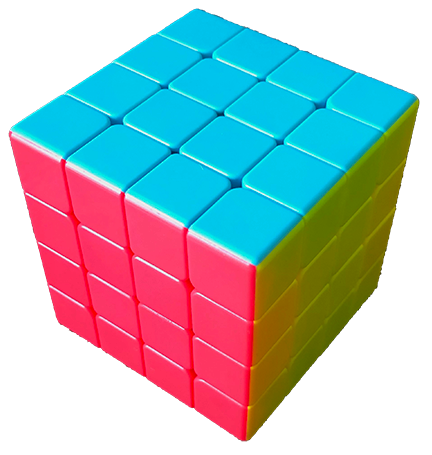
\includegraphics[height=1.6in,angle =5,origin=c]{cube.png}
\hspace{0.75in}
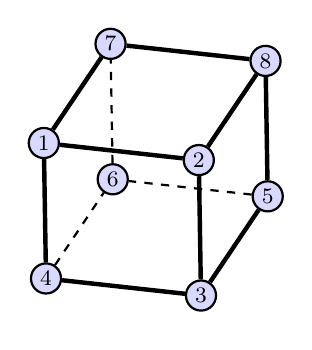
\begin{tikzpicture}[vertex/.style={circle,draw=black,fill=blue!15,thick,inner sep=1.5pt},ultra thick,rotate around x=15,rotate around y=-3,rotate around z=-5,scale = 1,baseline=-55pt]
\footnotesize
\begin{scope}
\node[vertex] (v4) at (-1,-1,1) {$4$};
\node[vertex] (v1) at (-1,1,1) {$1$};
\node[vertex] (v2) at (1,1,1) {$2$};
\node[vertex] (v3) at (1,-1,1) {$3$};
\node[vertex] (v6) at (-1,-1,-1) {$6$};
\node[vertex] (v7) at (-1,1,-1) {$7$};
\node[vertex] (v8) at (1,1,-1) {$8$};
\node[vertex] (v5) at (1,-1,-1) {$5$};
\end{scope}

\draw (v1) -- (v2) -- (v3) -- (v4) -- (v1);
\draw (v1) -- (v7) -- (v8) -- (v2);
\draw (v3) -- (v5) -- (v8);
\draw[dashed,thick] (v4) -- (v6) -- (v7);
\draw[dashed,thick] (v5) -- (v6);
\end{tikzpicture}
\end{center}

Note that $\symcube$ also acts faithfully on the $6$ faces as well as on the $12$ edges, so we could have instead chosen to label the faces or edges to view $\symcube$ as a subgroup of $\Sym(6)$ or $\Sym(12)$. However, for now, let's think in terms of the action on the vertices.

Rotating clockwise by $90^\circ$ around the axis running through the centers of faces $\{1,2,3,4\}$ and $\{5,6,7,8\}$, we get the permutation $\alpha = (1234)(5678)$. Performing $\alpha$ twice (i.e.~rotation about the same axis by $180^\circ$) yields the permutation $\alpha^2 = (13)(24)(57)(68)$. A third application of $\alpha$ results in $\alpha^3 = (1432)(5876)$, and  $\alpha^4 = \id$. Performing similar rotations around the axes running through the center of the other two pairs of opposite faces, yields $6$ more rotational symmetries, bringing our total thus far to $10$: $\id$, $3$ of ``shape'' $(13)(24)(57)(68)$, and $6$ of ``shape'' $(1234)(5678)$.

And there are more. Consider holding a pair of antipodal vertices, like $1$ and $5$. Let $D_1$ denote the diagonal line (running through the interior of the cube) connecting  $1$ and $5$. Rotating the cube by $120^\circ$ clockwise around $D_1$ gives the permutation $\gamma = (247)(683)$, and rotating by $240^\circ$ (or $-120^\circ$), yields $\gamma^2 = (274)(638)$. Considering the remaining three diagonals as well, we add $8$ permutations of shape $(247)(683)$ to our list of rotational symmetries, bringing our total thus far to $18$. 

And there are still more: we can rotate by $180^\circ$ around the axis connecting the midpoint of opposite edges of the cube. For example, rotating about the line connecting the midpoints of edges $\{1,4\}$ and $\{5,8\}$ yields the permutation $\beta = (14)(58)(26)(37)$. This produces $6$ more rotational symmetries (including $\beta$) of shape $(14)(58)(26)(37)$, and our total is now $24$. Have we found all rotational symmetries?  We could indeed construct a direct  argument that we have found them all, but just having a complete list of the symmetries is not the end of the story. We typically also want to know more about the ``structure'' of the  group itself.

To better understand $\rsymcube$, let's change our point of view slightly. Perhaps we've noticed something about how the symmetries treat antipodal (i.e.~opposite) vertices. For example,  once we know where a given symmetry sends the vertex $1$, we automatically know where $5$ must be sent. In short, any symmetry of the cube (rotational or not), must move a pair of antipodal vertices to a (perhaps same) pair of antipodal vertices. This can be used to show that $\symcube$ acts on the $4$ diagonals of the cube (pictured below). 
\begin{center}
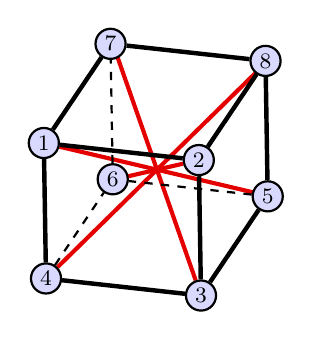
\begin{tikzpicture}[vertex/.style={circle,draw=black,fill=blue!15,thick,inner sep=1.5pt},ultra thick,rotate around x=15,rotate around y=-3,rotate around z=-5,scale = 1]
\footnotesize
\begin{scope}
\node[vertex] (v4) at (-1,-1,1) {$4$};
\node[vertex] (v1) at (-1,1,1) {$1$};
\node[vertex] (v2) at (1,1,1) {$2$};
\node[vertex] (v3) at (1,-1,1) {$3$};
\node[vertex] (v6) at (-1,-1,-1) {$6$};
\node[vertex] (v7) at (-1,1,-1) {$7$};
\node[vertex] (v8) at (1,1,-1) {$8$};
\node[vertex] (v5) at (1,-1,-1) {$5$};
\end{scope}

\draw (v1) -- (v2) -- (v3) -- (v4) -- (v1);
\draw (v1) -- (v7) -- (v8) -- (v2);
\draw (v3) -- (v5) -- (v8);
\draw[dashed,thick] (v4) -- (v6) -- (v7);
\draw[dashed,thick] (v5) -- (v6);
%Diagonals
\begin{pgfonlayer}{background}
\begin{scope}[red!90!black, line width = 1.5]
\foreach \x in {1,2,3,4} {
\tikzmath{\y = \x + 4;}
\draw (v\x) -- ([xshift=-5]v\y);
}
\end{scope}
\end{pgfonlayer}

\end{tikzpicture}
\end{center}

Let's use the notation $D_i$ for the diagonal line connecting vertex $i$ to $i+4$ (so  $D_i$ connects vertices that are equal modulo $4$). Our comment before is that $\symcube$ acts on the set $\mathcal{D} = \{D_1, D_2, D_3, D_4\}$. However, the action of $\symcube$ is \emph{not} faithful on $\mathcal{D}$. Indeed, there is a very special reflection that takes each vertex to the antipodal vertex; let's call this antipodal reflection $\rho$.  Then $\rho$ fixes every diagonal, so $\rho$ and $\id$ have the same action on $\mathcal{D}$. However, $\rsymcube$ does  act faithfully on $\mathcal{D}$: one can argue geometrically that the only rotational symmetry fixing all four diagonals is the identity. Thus, we may view $\rsymcube$ as a subgroup of $\Sym(\{D_1, D_2, D_3, D_4\})$. To simplify notation, let's forget about the $D$, and just label the diagonals $1,2,3,4$. In doing so, we may now view $\rsymcube$ as a subgroup of $\Sym(4)$. Let's revisit some of the symmetries from before and see how they permute the diagonals. 

\begin{center}
\small
\tabulinesep = 1.2mm
\begin{tabu} to 5in {X[0.4,c,m]|[1pt]X[c,m]|[1pt]X[c,m]}
Symmetry  & Permuting the vertices  & Permuting the diagonals \\ \tabucline[2pt]{-}
$\alpha$ & $(1234)(5678)$ & $(1234)$ \\ \tabucline[1pt]{-}
$\alpha^2$ & $(13)(24)(57)(68)$ & $(13)(24)$ \\ \tabucline[1pt]{-}
$\gamma$ & $(247)(683)$ & $(243)$ \\ \tabucline[1pt]{-}
$\beta$ & $(14)(58)(26)(37)$ & $(14)$ \\ \tabucline[1pt]{-}
$\rho \notin \rsymcube$ & $(15)(26)(37)(48)$ & $\id$ 
\end{tabu}
\end{center}

Now, remember that we found $24$ rotational symmetries. If we view $\rsymcube \subseteq \Sym(4)$ (permuting the diagonals), then as $|\Sym(4)| = 24$, it must be that $\rsymcube = \Sym(4)$. And this gives a nice description of $\rsymcube$ as realizing all possible permutations of the $4$ diagonals (in a way that different elements of $\rsymcube$ represent different permutations of the diagonals). 

And what about $\symcube$? It turns out that if $\tau \in \symcube$, then either $\tau \in \rsymcube$ or $\tau = \sigma\rho$ for some $\sigma \in \rsymcube$ (with $\rho$ the antipodal reflection). In other words, every symmetry of the cube is either a rotational symmetry (which we understand in terms of how it permutes the diagonals) or it is a composition of a rotational symmetry with the antipodal reflection. Moreover, for each $\sigma \in \rsymcube$, $\sigma \rho = \rho\sigma$, which (in group theoretic notation) implies that $\symcube = \rsymcube \times \{\id, \rho\} \cong \Sym(4) \times \mathbb{Z}_2$.
\end{example}


% % % % % % % % % % % % % % % % % % % % % % % % % % % % % % % % % % % % % % % % % % % % % % % % % 
% Subsection
% % % % % % % % % % % % % % % % % % % % % % % % % % % % % % % % % % % % % % % % % % % % % % % % % 
\subsection{Orbits and stabilizers}

\begin{example}\label{exam:Icosa}
Let's look at the symmetries of a regular icosahedron. (The Rubik-esque version of this is the \href{https://en.wikipedia.org/wiki/Dogic}{Dogic} pictured below.) Let $\rsymicosa$ denote the set of rotational symmetries. Notice that $\rsymicosa$ acts faithfully on the $12$ vertices of the icosahedron, so after labeling the vertices (as below), we can view $\rsymicosa$ as a subgroup of $\Sym(12)$. 

\begin{center}
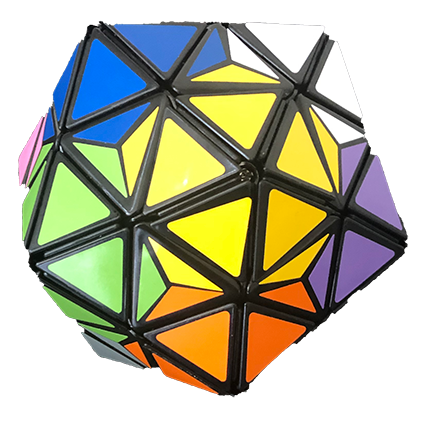
\includegraphics[height=2in,angle =15,origin=c]{icosahedron.png}
\hspace{0.75in}
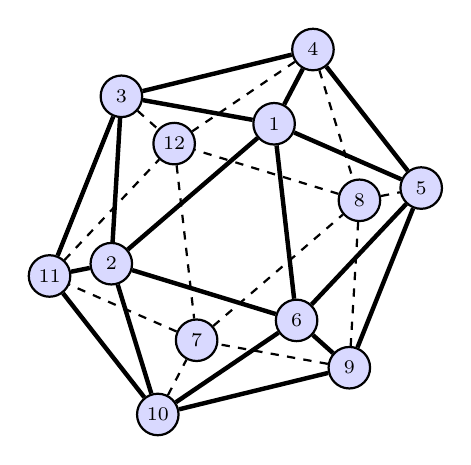
\begin{tikzpicture}[vertex/.style={circle,draw=black,fill=blue!15,thick,inner sep=1.5pt,minimum size=15pt},line width = 1.2,line join=round,rotate around x=0,rotate around y=-50,rotate around z=20,scale = 1.2]
\scriptsize

\tikzmath{\a = 1; \z = \a*(1/2 + sqrt(5)/2);}

\node[vertex](A) at (0,\z,\a) {$3$};
\node[vertex](B) at (0,\z,-\a) {$4$};
\node[vertex](C) at (0,-\z,\a) {$10$};
\node[vertex](D) at (0,-\z,-\a) {$9$};
\node[vertex](E) at (\a,0,\z) {$2$};
\node[vertex](F) at (\a,0,-\z) {$5$};
\node[vertex](G) at (-\a,0,\z) {$11$};
\node[vertex](H) at (-\a,0,-\z) {$8$};
\node[vertex](I) at (\z,\a,0) {$1$};
\node[vertex](J) at (\z,-\a,0) {$6$};
\node[vertex](K) at (-\z,\a,0) {$12$};
\node[vertex](L) at (-\z,-\a,0)  {$7$};

%\draw[red] (0,0,-3) -- (0,0,3);
%\draw[blue] (0,-3,0) -- (0,3,0);

\draw[dashed, thick]    
(B) -- (H) -- (F) 
(D) -- (L) -- (H) -- (D) 
(K) -- (L) -- (H) -- (K)
(K) -- (L) -- (G) -- (K)
(C) -- (L) (B)--(K) (A)--(K)
;
        
\draw[ultra thick]
(A) -- (I) -- (B) -- (A) 
(F) -- (I) -- (B) -- (F) 
(F) -- (I) -- (J) -- (F)
(F) -- (D) -- (J) -- (F)
(C) -- (D) -- (J) -- (C)
(C) -- (E) -- (J) -- (C)
(I) -- (E) -- (J) -- (I)
(I) -- (E) -- (A) -- (I)
(G) -- (E) -- (A) -- (G)
(G) -- (E) -- (C) -- (G)
; 
\end{tikzpicture}
\end{center}

This time, we'll just try to count the number of symmetries in $\rsymicosa$ and leave the  determination of which permutations are in $\rsymicosa$ (and $\symicosa$) as an exercise. Let $\sigma\in \rsymicosa$ denote an arbitrary rotational symmetry. In two-line notation, $\sigma$ has the form
\[\sigma = \begin{pmatrix}
1 & 2 & 3 & \cdots & 12\\
\sigma(1) & \sigma(2) & \sigma(3) & \cdots & \sigma(12)\\
\end{pmatrix}\]
To count $\rsymicosa$, let's count the possible ways we can fill in the bottom row of the two-line notation for $\sigma$. Notice that there are rotations taking vertex $1$ to any other vertex (including $1$), so there are $12$ possibilities for $\sigma(1)$. 

Now assume that we have chosen $\sigma(1)$; how many possibilities remain for $\sigma(2)$?  Notice that when counting the possibilities for $\sigma(2)$, the actual value of $\sigma(1)$ does not matter, so without loss of generality, we may assume that $\sigma(1)=1$, i.e.~$\sigma$ fixes $1$. Since $2$ is connected to $1$ by an edge and $\sigma$ fixes $1$, $\sigma(2)$ must also be connected to $1$ by an edge, and we see that there are $5$ possibilities for $\sigma(2)$, which  correspond to rotations of the icosahedron about the line connecting $1$ to its antipodal vertex $7$. 

Thus far, we found that there are $12$ possibilities for $\sigma(1)$, and that once given $\sigma(1)$, there are $5$ possibilities for $\sigma(2)$. Now assume that we know $\sigma(1)$ and $\sigma(2)$. What about $\sigma(3)$? Let's keep assuming that $\sigma(1)=1$. Also, when counting possibilities for $\sigma(3)$, it does not matter which of the $5$ vertices we choose for $\sigma(2)$, so let's assume that $\sigma(2) = 2$  (again without any loss of generality). But if $\sigma$ fixes the vertices $1$ and $2$, then the axis of rotation for $\sigma$ passes through the edge $\{1,2\}$. However, the only rotation fixing an edge of the icosahedron is the identity, meaning that the only choice for $\sigma(3) = 3$ and in fact that $\sigma(k) = k$ for all $k\ge 3$. 

In summary, there are $12$ possibilities for $\sigma(1)$, from which $5$ possibilities remain for $\sigma(2)$, and then only one choice remains for each $\sigma(k)$ with $k\ge 3$. Thus, $|\rsymicosa| = 60$.
\end{example}

In Example~\ref{exam:Icosa}, we encountered the need to discuss all possible vertices to which $\rsymicosa$ can take vertex $1$. This is an important concept for all permutation groups, and so we give it a name: the \emph{orbit} of $1$ under $\rsymicosa$. We also had need to consider all symmetries in $\rsymicosa$ that fixed the  vertex $1$. This is an equally important concept that we also name:  the \emph{stabilizer} of $1$ in $\rsymicosa$. Here are the proper definitions.

\begin{definition}
Let $G$ act on $X$, and let $y\in X$. 
\begin{itemize}
\item The \textbf{orbit of $y$ under $G$} is defined by $\Orb_G(y) = \{ x\in X \mid \text{$x = g\cdot y$ for some $g\in G$}\}$.
\item The \textbf{stabilizer of $y$ in $G$} is defined by $G_y = \{ g\in G \mid g \cdot y = y\}$.
\end{itemize}
When considering stabilizers of stabilizers, we use notation $G_{y_1,y_2}$ in place of $(G_{y_1})_{y_2}$.
\end{definition}

\begin{example}
Let's revisit Example~\ref{exam:Icosa} and record our findings using the language of orbits and stabilizers. Set $G = \rsymicosa$. 

We first found that $\Orb_G(1) = \{1,2,\dots, 12\}$. In fact, no matter which vertex $k$ we choose, $\Orb_G(k) = \{1,2,\dots, 12\}$. Thus, $G$ has only one orbit on the vertices, consisting of them all.

Next, instead of studying orbits with respect to $G$, we changed to considering the stabilizer $G_1$. Here we found that $\Orb_{G_1}(2) = \{2,3,4,5,6\}$. We could also ask where $G_1$ could take vertices other than $2$. Since $G_1$ fixes $1$, $\Orb_{G_1}(1) = \{1\}$. As $G_1$ also fixes the antipodal vertex $7$, $\Orb_{G_1}(7) = \{7\}$. There are various other vertices to consider, and, for example, $\Orb_{G_1}(8) = \{8,9,10,11,12\}$. Here is the complete list of orbits for $G_1$: \[\{1\}, \{7\}, \{2,3,4,5,6\}, \{8,9,10,11,12\}.\]

Finally, we considered the stabilizer $G_{1,2}$. This time we found that $G_{1,2}$ must fix every vertex, so for each vertex $k$, $\Orb_{G_{1,2}}(k) = \{k\}$.
\end{example}

In Example~\ref{exam:Icosa}, not only did we consider orbits and stabilizers, but we also combined information about the two in order to count the size of the set being acted upon. The next theorem formalizes that process. In the statement of the theorem we use the notation $|A|$ to denote the cardinality (i.e.~the ``size'') of the set $A$.

\begin{theorem*}
Let $G$ act on $X$, and let $x\in X$. Then $|G| = |\Orb_G(x)|\cdot |G_x|$.
\end{theorem*}
\begin{proof}
We define a function $\phi: G \rightarrow \Orb_G(x)$ via $\phi(g) = g\cdot x$, so  $g\cdot x =  y \iff \phi(g) = y$. By definition of $\Orb_G(x)$, $\phi$ maps \emph{onto} $\Orb_G(x)$, but $\phi$ is  not likely one-to-one. For example, every element of $G_x$ maps to $x$. Here is a picture.
\begin{center}
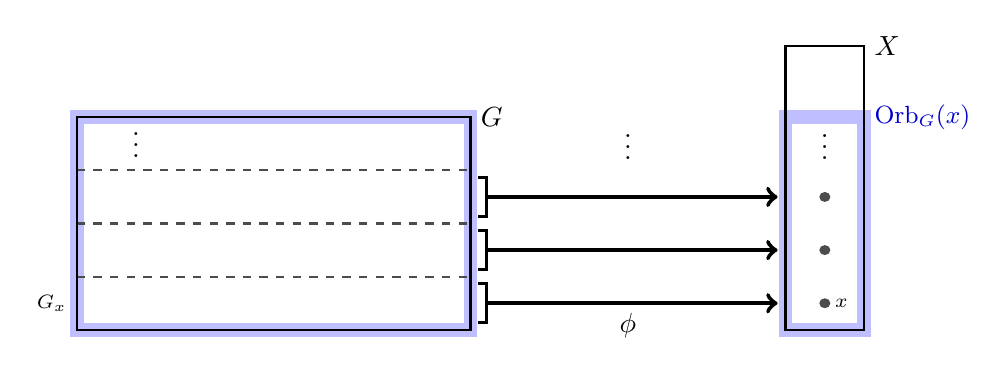
\begin{tikzpicture}[thick, yscale = 0.9]
\draw[blue!25, line width = 5] (0,0)--(5,0)--(5,3)--(0,3)--cycle;
\foreach \i in {1,2,3} {
\draw[dashed, black!70] (0,\i*0.75) -- (5,\i*0.75);
\draw[black, line width = 1.2] (5.1,{(\i-1)*0.75+0.65}) -- (5.2,{(\i-1)*0.75+0.65}) -- (5.2,{(\i-1)*0.75+0.1})-- (5.1,{(\i-1)*0.75+0.1});
\draw[black, ultra thick,->] (5.2,{(\i-1)*0.75+0.75/2}) -- (8.9,{(\i-1)*0.75+0.75/2});
}
\node at (7,{3*0.75+0.45}) {$\vdots$};
\node[anchor = north] at (7,{0.75/2}) {$\phi$};
\node[black, anchor =0] at (0,0.75/2) {\scriptsize$G_x$};
%\node[black] at (0.75,{0.75+0.75/2}) {\scriptsize${gG_x}$};
\node[black] at (0.75,{1.5+0.75/2}) {};
\node[black] at (0.75,{2.35+0.75/2}) {$\vdots$};
\node[anchor = west] at (5,3) {$G$};
\draw (0,0)--(5,0)--(5,3)--(0,3)--cycle;
\draw[black, line width = 1.2] (5.1,{0.75+0.65}) -- (5.2,{0.75+0.65}) -- (5.2,{0.75+0.1})-- (5.1,{0.75+0.1});
\begin{scope}[shift = {(9,0)}]
\draw[blue!25, line width = 5] (0,0)--(1,0)--(1,3)--(0,3)--cycle;
\foreach \i in {1,2,3} {\fill[black!70] (0.5,{(\i-1)*0.75+0.75/2}) circle (2pt);}
\node[anchor = west] at (0.5,{0.75/2}) {\scriptsize$x$};
%\node[anchor = west] at (0.5,{0.75+0.75/2}) {\scriptsize$y$};
\node[anchor = west] at (0.5,{2*0.75+0.75/2}) {};
\node[black] at (0.5,{3*0.75+.45}) {$\vdots$};
\node[anchor = west] at (1,4) {$X$};
\node[blue!80!black,anchor = west] at (1,3) {\small$\Orb_G(x)$};
\draw (0,0)--(1,0)--(1,4)--(0,4)--cycle;
\end{scope}
\end{tikzpicture}
\end{center}

For a given $g\in G$, let's count the number of $h\in G$ such that $\phi(g) = \phi(h)$. Notice that \[\phi(g) = \phi(h) \iff g\cdot x = h\cdot x \iff x = g^{-1}h\cdot x \iff g^{-1}h\in G_x \iff h\in gG_x,\]
where we use the notation $gG_x$ to denote the set $\{ga \mid a\in G_x\}$. So,  counting the number of $h$ such that $\phi(g) = \phi(h)$ is the same as determining the cardinality of  $gG_x$. 
Now notice that for all $a,b\in G_x$, 
\[ga = gb \iff a = g^{-1}gb \iff a = b,\]
which tells us that counting the number of $ga\in gG_x$ is the same as counting the number of $a\in G_x$. Thus, $|gG_x| = |G_x|$, and crucially, this does \emph{not} depend on the choice of $g$. So each ``fiber'' in the picture above has the same size, which is $|G_x|$. 

We conclude that for every $y \in \Orb_G(x)$, there are precisely $|G_x|$-many elements of $G$ that map to $y$. Thus, $|G| = |\Orb_G(x)|\cdot |G_x|$.
\end{proof}

\begin{example}
Let's revisit Example~\ref{exam:Icosa} yet again. Set $G = \rsymicosa$. 

The previous theorem says that $|G| = |\Orb_G(1)|\cdot |G_1|$. Since we know that $\Orb_G(1) = \{1,2,\dots, 12\}$, we get that $|G| = 12\cdot |G_1|$. 

We can now apply the same theorem to $G_1$ to get that $|G_1| = |\Orb_{G_1}(2)|\cdot |G_{1,2}|$, so as $\Orb_{G_1}(2) = \{2,3,4,5,6\}$, $|G_1| = 5\cdot |G_{1,2}|$. Combining with what we've already learned, we get that $|G| = 12\cdot 5 \cdot |G_{1,2}|$.

And finally, we also know that $G_{1,2}$ must fix every vertex, but the only element of $G$ fixing all vertices is the identity. Thus, $G_{1,2} = \{\id\}$, so $|G_{1,2}| = 1$. Thus,  $|G| = 12\cdot 5 \cdot 1 = 60$.
\end{example}

% % % % % % % % % % % % % % % % % % % % % % % % % % % % % % % % % % % % % % % % % % % % % % % % % 
% % % % % % % % % % % % % % % % % % % % % % % % % % % % % % % % % % % % % % % % % % % % % % % % % 
% Section
% % % % % % % % % % % % % % % % % % % % % % % % % % % % % % % % % % % % % % % % % % % % % % % % % 
% % % % % % % % % % % % % % % % % % % % % % % % % % % % % % % % % % % % % % % % % % % % % % % % % 
\section{Degrees of symmetry}\label{S:multipletrans}

Which would you say is ``more symmetric'': a regular tetrahedron or a cube? Why? 
A first thought may be that an object is more symmetric if it has more symmetries. With that point of view, a cube would be more symmetric than a tetrahedron since our work in Examples~\ref{exam:Tetra} and \ref{exam:Cube} implies that $|\symcube| = 48 > 24 = |\symtetra|$. However, this approach seems to privilege the cube simply because it has more vertices. 

Let's work towards another approach to measuring symmetry. We saw that there is a symmetry taking any vertex of the tetrahedron to any other, and the same is true for a cube. %As such, we may think of the vertices of the tetrahedron (respectively the cube) as being indistinguishable from one another. 
But now, what if we ask about pairs of vertices. Notice that any two vertices of a tetrahedron can be simultaneously moved to any other two vertices. However, the same is \emph{not} true for the cube: a pair of antipodal vertices can never be simultaneously moved to a pair of non-antipodal vertices. And this difference suggests that we might view the tetrahedron as being more symmetric than the cube. Let's formalize this idea.

\begin{notation}
For $X$ a set, $X^n$ denotes the set of all $n$-tuples with entries from $X$, and $X^{(n)}$ denotes the subset of $X^n$ consisting of tuples with distinct entries, i.e. \[X^{(n)} = \{(x_1,\ldots,x_n) \in X^n \mid \text{$x_i \neq x_j$ for all $i\neq j$}\}.\]
\end{notation}

For example, $(1,2,3,2)\notin \mathbb{Z}^{(4)}$ because of the repeated $2$, but $(1,2,3,7)\in \mathbb{Z}^{(4)}$ as there is no repetition in the coordinates. 

\begin{remark*}
If $G$ acts on $X$, then $G$ acts coordinatewise on both $X^{n}$ and $X^{(n)}$ via the rule \[g\cdot(x_1,\ldots,x_n) = (g\cdot x_1,\ldots,g\cdot x_n).\] 
\end{remark*}

\begin{definition*}
We say that an action of $G$ on $X$ is \textbf{transitive} if $G$ has only one orbit on $X$. More generally, we say the action is \textbf{$k$-transitive} if $G$ has only one orbit on $X^{(k)}$ (with respect to the coordinatewise action).
\end{definition*}

\begin{example}
Let's revisit Examples~\ref{exam:Tetra} and \ref{exam:Cube} through the lens of $k$-transitivity. 

The comment above that any two  (distinct) vertices of a tetrahedron can be moved to any other two (distinct) vertices is stating that the action of $\symtetra$ on the vertices of  the tetrahedron is $2$-transitive. In fact, such pairs of vertices can be moved using a rotation, so $\rsymtetra$ also acts $2$-transitively on the vertices. And more is true: $\symtetra$ in fact acts $4$-transitively on the vertices. 

As for the cube, $\symcube$ and $\rsymcube$ act transitively on the vertices, but neither act $2$-transitively. However, $\rsymcube$ does act $4$-transitively on the four diagonals of the cube. 
\end{example}

\begin{example}
If $X = \{1,\ldots,n\}$, then it is fairly straightforward to verify that $\Sym(n)$ acts $n$-transitively on $X$, and it is ever so slightly less-straightforward to check that the action of $\Alt(n)$ is $(n-2)$-transitive but not $(n-1)$-transitive. 
\end{example}

Although we have seen some examples of \textbf{multiply transitive} actions (i.e.~$k$-transitive actions for $k\ge 2$), it turns our that this is relatively rare. And as one might expect, it becomes even rarer to find $k$-transitive actions as $k$ increases, which is to say that highly symmetric objects are rare. 

Let's meet some new permutation groups as we continue to investigate $k$-transitivity. 

\begin{example}\label{exam.AGL1R}
Let's take a look at a particular group of permutations on $\mathbb{R}$. Specifically, we will consider the set of invertible (affine) linear functions: \[\AGL_1(\mathbb{R}) = \{ f \in \Sym(\mathbb{R}) \mid \text{$f(x) = mx+b$ for some $m,b\in \mathbb{R}$ with $m\neq 0$}\}.\]
It can be checked that $\AGL_1(\mathbb{R})$ satisfies the necessary closure axioms to be a permutation group on $\mathbb{R}$. Let's determine how transitive this action is.

Is the action transitive? Yes. For all $r,s\in \mathbb{R}$, the translation $f(x) = x + (s-r)$ is in $\AGL_1(\mathbb{R})$ and $f(r) = s$, so $\AGL_1(\mathbb{R})$ has a single orbit on $\mathbb{R}$.
What about $2$-transitivity? Let's consider $(r_1,r_2),(s_1,s_2)\in \mathbb{R}^{(2)}$. We need to determine if there exists $f\in \AGL_1(\mathbb{R})$ such that $f\cdot (r_1,r_2) = (s_1,s_2)$, which translates to $f(r_1) = s_1$ and $f(r_2) = s_2$. If we graph the points $(r_1, s_1)$ and $(r_2, s_2)$ (remembering that $r_1 \neq r_2$ and $s_1 \neq s_2$ by definition of $\mathbb{R}^{(2)}$), we have something like the following:
\begin{center}
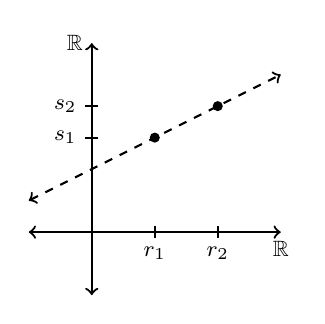
\begin{tikzpicture}[thick, scale = .8]
\footnotesize
\draw[<->] (-1,0) -- (3,0) node[anchor = 90] {$\mathbb{R}$};
\draw[<->] (0,-1) -- (0,3) node[anchor = 0] {$\mathbb{R}$};
\draw (1,.1)-- (1,-.1) node[anchor = 90] {$r_1$};
\draw (.1,1.5)-- (-.1,1.5)  node[anchor = 0] {$s_1$};
\draw (2,.1)-- (2,-.1)  node[anchor = 90] {$r_2$};
\draw (.1,2)-- (-.1,2)  node[anchor = 0] {$s_2$};
\draw[dashed, <->] (-1,0.5) -- (3,2.5); 
\fill (1,1.5) circle (.08);
\fill (2,2) circle (.08);
\end{tikzpicture}
\end{center}
The function representing the line connecting the two points will take $r_1$ to $s_1$ and $r_2$ to $s_2$, which is what we want, so the action is indeed $2$-transitive.

Could it be $3$-transitive? If it were,  there would have to be some $f\in \AGL_1(\mathbb{R})$ such that $f\cdot (0,1,2) = (0,1,3)$, meaning that $f(0) = 0$, $f(1) = 1$, and $f(2) = 3$. Writing $f(x) = mx+b$, $f(0) = 0$ implies $b=0$, and then $f(1) = 1$ implies $a = 1$. Thus $f$ is the identity function $f(x) = x$, but then there is no way that $f(2) = 3$. So no, the action is not $3$-transitive.
\end{example}

In Example~\ref{exam.AGL1R}, we considered the group of invertible linear functions from $\mathbb{R}$ to $\mathbb{R}$, but we used very little specific knowledge of $\mathbb{R}$ in the example. For example, we would have reached the same conclusion for invertible linear functions from $\mathbb{Q}$ to $\mathbb{Q}$. As such, we will define $\AGL_1(F)$ where $F$ is any \href{https://en.wikipedia.org/wiki/Field_(mathematics)}{field}; roughly, a \textbf{field} is a mathematical structure were there are ``well-behaved'' notions of addition and multiplication, as well as additive and multiplicative inverses. Examples of fields include $\mathbb{Q}$, $\mathbb{R}$, and $\mathbb{C}$, but not $\mathbb{Z}$ because of the lack of multiplicative inverses for most elements. 

\begin{definition*}
For $F$ a field, we define \[\AGL_1(F) = \{ f \in \Sym(F) \mid \text{$f(x) = mx+b$ for some $m,b\in F$ with $m\neq 0$}\}.\]
\end{definition*}

\begin{remark*}
Essentially the same proof we gave in Example~\ref{exam.AGL1R} shows that, for any field $F$, $\AGL_1(F)$ acts $2$-transitively on $F$. Moreover, if $|F| \ge 4$, then the action is \emph{not} $3$-transitive. 
\end{remark*}

The group $\AGL_1(F)$ can be generalized in (at least) a couple of ways. One way is to directly adapt the definition to give functions from the vector space $F^n$ to itself by considering functions $f(x) = mx+b$ where $m$ is an $n\times n$ matrix and $b$ an $n$-vector. 

\begin{definition*}
For $F$ a field, let $\GL_{n}(F)$ denote all \emph{invertible} $n\times n$ matrices with entries from $F$, and define
\[\AGL_n(F) = \{ f \in \Sym(F^n) \mid \text{$f(\bar{x}) = A\bar{x}+\bar{b}$ for some $A\in \GL_{n}(F)$ and some $\bar{b} \in F^n$}\}.\]
We refer to $\AGL_n(F)$ as the \textbf{affine general linear group} of degree $n$.
\end{definition*}

\begin{remark*}
We won't explore $\AGL_n(F)$ much here, but it's worth mentioning that---just like $\AGL_1(F)$---each permutation group in this family (for all choices of $n$ and $F$) acts  $2$-transitively on the vector space $F^n$, and provided $|F| \ge 4$, the action is not $3$-transitive.
\end{remark*}

Let's now take at another way to generalize the construction of $\AGL_1(F)$. This time we will encounter a family of permutation groups that are typically $3$-transitive but not $4$-transitive.

\begin{example}\label{exam.PGL1R}
In Example~\ref{exam.AGL1R}, we looked at certain functions on the line $\mathbb{R}$; this time we will work with the projective line $\Proj^1(\mathbb{R}) = \mathbb{R} \cup \{\infty\}$. Right now, $\infty$ is just another symbol we are adding to the set $\mathbb{R}$, but we can think of $\Proj^1(\mathbb{R})$ as a circle where $\infty$ connects the positive and negative ``ends'' of the real line.
\begin{center}
\begin{tikzpicture}[thick, scale = 0.8]
\footnotesize
\begin{scope}
\draw[<->] (-pi,0) -- (pi,0);
\draw (0,.1) -- (0,-.1)  node[anchor = 90] {$0$};
\node at (0,1) {$\mathbb{R}$};
\end{scope}
\begin{scope}[shift = {(6,0)}]
\draw[<->] plot[samples=100,domain=-263:83,smooth]  ({cos(\x)},{sin(\x)+1});
\draw (0,.1) -- (0,-.1)  node[anchor = 90] {$0$};
\node[anchor = -90] at (0,2) {$\infty$};
\fill (0,2) circle (.08);
\node at (0,1) {$\Proj^1(\mathbb{R})$};
\end{scope}
\end{tikzpicture}
\end{center}

We now define a special collections of permutations of the projective line, namely the so-called \textbf{factional linear transformations}:
\[\PGL_2(\mathbb{R}) = \left\{ f \in \Sym(\Proj^1(\mathbb{R})) \mid \text{$f(x) = \frac{ax+b}{cx+d}$ for $a,b,c,d\in \mathbb{R}$ with $ad-bc\neq 0$}\right\}.\]

In order for a function of the form $f(x) = \frac{ax+b}{cx+d}$ to be fully defined  from $\Proj^1(\mathbb{R})$ to $\Proj^1(\mathbb{R})$, we need to make sense of a couple values: $f(\infty) = \frac{a}{c}$ and $f\left(\frac{-d}{c}\right) = \infty$. The first can be thought of via the arithmetic that $a\cdot\infty+b = a\cdot\infty$, $c\cdot\infty+d = c\cdot\infty$, and $\frac{a\cdot\infty}{c\cdot\infty} = \frac{a}{c}$; the second one is just expressing that $\frac{e}{0} = \infty$ for each nonzero $e\in \mathbb{R}$.

Note that $\AGL_1(\mathbb{R}) \subset \PGL_2(\mathbb{R})$ by using $c=1$ and $d = 0$ in the definition above. Moreover, every element of $\AGL_1(\mathbb{R})$ fixes $\infty$, and in fact, $\AGL_1(\mathbb{R})$ is equal to the stabilizer of $\infty$ in $\PGL_2(\mathbb{R})$. Also note that the function $i(x) = \frac{1}{x} \in \PGL_2(\mathbb{R})$, where $i(0) = \infty$ and $i(\infty) = 0$. If we scale the circle above so that $-1$ and $1$ are the endpoints of the horizontal diameter, then the function $i(x)$ can be viewed as a reflection over that diameter.

Let's now show that $\PGL_2(\mathbb{R})$ acts $3$-transitively on $\Proj^1(\mathbb{R})$.

\end{example}










\vfill

\begin{center}
    \textsc{To be continued}\dots
\end{center}

\newpage

\bibliographystyle{alpha}
\bibliography{PermutationGroupsNotes}
\end{document}

